
\documentclass[xcolor=table]{beamer}

% for fancy Mike style table
 \usepackage[table]{xcolor} 
 \usepackage{multirow}
\usepackage{textpos}
\usepackage{helvet}
\usepackage{caption}
\usepackage{changepage}
\usepackage{algorithmic}
\usepackage{array}
\setbeamerfont{caption}{size = \footnotesize}
\usepackage{multicol}
\usepackage{setspace}

% useful packages for including code
\usepackage{listings}
\usepackage{color}
\lstset{breaklines}

% package for drawing graphs
\usepackage{tikz}
\usetikzlibrary{positioning}

\definecolor{charlesBlue}{RGB}{100, 155, 255}
\definecolor{charlesBlue2}{RGB}{0, 155, 255}
\definecolor{MRGGreen}{rgb}{0, 0.350, 0.200}
\usecolortheme{default}

% References
%\bibliographystyle{apacite} 
\hypersetup{colorlinks = true, linkcolor={MRGGreen}, citecolor = black, urlcolor = blue}


% Custom colors for alerts and examples
\setbeamercolor{palette primary}{fg=MRGGreen}
\setbeamercolor{palette secondary}{fg=MRGGreen}
\setbeamercolor{palette tertiary}{bg= MRGGreen}
\setbeamercolor*{structure}{fg=MRGGreen}
\setbeamercolor{titlelike}{fg=black}

\lstset{
  basicstyle=\tiny \ttfamily,
  columns=fullflexible,
}


\begin{document} 

\begin{frame}
  \begin{center}
    {\Large IV} \\ \ \\ Population models
  \end{center}
\end{frame}

\begin{frame}
  
  Suppose our data can be pooled into groups.
  \begin{itemize}
    \item medical measurements are grouped by patients
    \item sport measurements are grouped by players
     \item people's voting intention can be grouped by states, social status, etc.
  \end{itemize}

\end{frame}


\begin{frame}
  
  \begin{figure}
    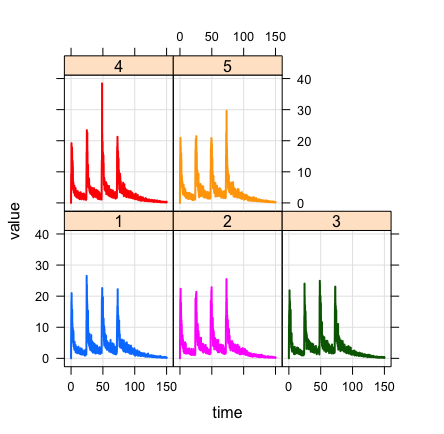
\includegraphics[width = 7.5cm]{../figures/Dosing_regimes.png}
  \end{figure}

  Simulated with \textit{mrgsolve} (\url{https://mrgsolve.github.io/})

\end{frame}

\begin{frame}

  With a hierarchical model, we can:
  \begin{itemize}
    \item do partial pooling.
    \item estimate how similar the groups are to one another.
    \item estimate individual parameters.
  \end{itemize}

\end{frame}

\begin{frame}
  \frametitle{Hierarchical model}
  
  $$\theta = (\theta_1, ..., \theta_L) \sim p(\theta | \theta_\mathrm{pop}) $$
  
  $$y = (y_1, ..., y_N) \sim p(y | \theta, x) $$
 

\end{frame}

\begin{frame}
  \frametitle{Hierarchical model}
  
  \begin{figure}
    \begin{center}
    \begin{tikzpicture}
    [
      Empty/.style={rectangle, draw=white!, fill=green!0, thick, minimum size=1mm},
      Gray/.style={rectangle, draw=black!, fill=gray!35, thick, minimum size=1mm},
      Round/.style={circle, draw=black!, fill=green!0, thick, minimum size=10mm},
    ]
    
    % Nodes
    \node[Empty] (theta) at (0, 0) {$\theta_\mathrm{pop}$};
    \node[Empty] (beta1) at (-3, -2) {$\theta_1$};
    \node[Empty] (beta2) at (-1, -2) {$\theta_2$};
    \node[Empty] (. . .) at (1, -2) {. . .};
    \node[Empty] (betaL) at (3, -2) {$\theta_L$};
    
    \node[Empty] (y1) at (-2.5, -4) {$y^2_1$};
    \node[Empty] (y2) at (-1.5, -4) {$y^2_2$};
    \node[Empty] (y. . .) at (-0.5, -4) {. . . };
    \node[Empty] (yN) at (0.5, -4) {$y^2_{n_2}$};
    
    % Lines
      \path [->, draw] (theta) -- (beta1);
      \path [->, draw] (theta) -- (beta2);
      \path [->, draw] (theta) -- (betaL);
      
      \path[->, draw] (beta2) -- (y1);
      \path[->, draw] (beta2) -- (y2);
      \path[->, draw] (beta2) -- (yN);

  \end{tikzpicture}
  \end{center}
  \end{figure}

\end{frame}

\begin{frame}
  \frametitle{Example 3: Hierarchical two compartment model}
  
  Likelihood function:
  \begin{eqnarray*}
    \log \theta & \sim & \mathrm{Normal}(\log \theta_\mathrm{pop}, \Omega) \\ \\
    \Omega & = & \left(\begin{array}{ccccc} 
                            \omega_1 & 0 & 0 & 0 & 0 \\
                            0 & \omega_2 & 0 & 0 & 0 \\
                            0 & 0 & \omega_3 & 0 & 0 \\
                            0 & 0 & 0 & \omega_4 & 0 \\
                            0 & 0 & 0 & 0 & \omega_5
                            \end{array} \right) \\ \\ \\
    \log (cObs) & \sim & \mathrm{Normal}\left(\log \left(\frac{y_2}{VC} \right), \sigma^2 \right)
  \end{eqnarray*}
  
\end{frame}

\begin{frame}

  \textit{\textcolor{MRGGreen}{Exercise 6}: Write, fit, and diagnose a hierarchical two
     compartment model for a population of 10 patients.
     Use \texttt{data/twoCptPop.data.r} and \texttt{twoCptPop.r}.}
     %
     \begin{itemize}
       \item \textit{Start by running 3 chains with 30 iterations.}
       \item \textit{Do you get any warning messages?}
     \end{itemize}
   
\end{frame}

\begin{frame}
  \frametitle{Divergent transitions}
  
   ``There were 29 divergent transitions after warmup.''
   
   \begin{itemize}
     \item A divergent transition occurs when we fail to accurately compute
     a Hamiltonian trajectory.
     \item This is because we \textit{approximate} trajectories.
     \item Our sampler may not be refined enough to explore the entire typical set.
   \end{itemize}

\end{frame}

\begin{frame}
  \frametitle{Divergent transitions}
  
  Consider the following hierarchical model:

  \begin{eqnarray*}
    \alpha_i &\sim& \mathrm{Normal}(\mu, \sigma)  \\
    y_i &\sim& p(y | \alpha_i)
  \end{eqnarray*}

\end{frame}

\begin{frame}
  \frametitle{Divergent transitons}
  
  $$ \alpha_i \sim \mathrm{Normal}(\mu, \sigma) $$
  
  Fitting this model yields the following pairs plot:

  \begin{center}
    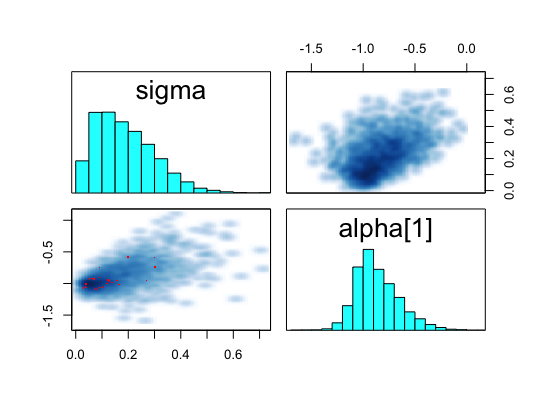
\includegraphics[width=5cm]{../figures/pairs_baseball2.png}
  \end{center}

\end{frame}

\begin{frame}

  \begin{itemize}
    \item This geometric shape is known as Neil's funnel \cite{Neil:2003}.
    \item Its interactions with HMC is described in \cite{Betancourt:2015}.
    \item It occurs in hierarchical models when we have sparse data and
    a centered prior.
  \end{itemize}

\end{frame}

\begin{frame}
  
  Proposition: reparametrize the model to avoid the funnel shape.
  We will do so by standardizing $\alpha$.
  
  $$ \alpha_{\mathrm{std}, i} := \frac{\alpha_i - \mu}{\sigma} $$
  
  Then
  
  $$ \alpha_\mathrm{std} \sim \mathrm{Normal}(0, 1)  $$
  
\end{frame}

\begin{frame}
  Then
    $$ \alpha_i = \mu + \sigma \alpha_{\mathrm{std}, i} $$
    
    Hence
      $$ y_i  \sim p(\mu + \sigma \alpha_{\mathrm{std}, i}) $$

   \ \\ \ \\
   \begin{itemize}
     \item Same data generating process; but how does this affect the geometry
     of the posterior?
   \end{itemize}

\end{frame}

\begin{frame}
  Our model is a little more complicated than the above example:
  \begin{itemize}
    \item a lot of parameters (100 +)!
    \item multiple population parameters and hierarchical structures.
    \item these parameters follow a log normal distribution (so we need
    a pairs plot with $\log \theta$).
  \end{itemize}

\end{frame}

\begin{frame}  
  \begin{center}
    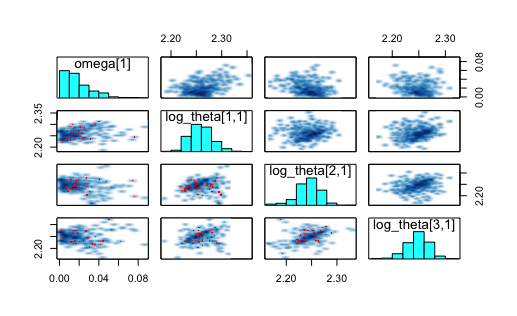
\includegraphics[width=9cm]{../figures/twoCptPairs1}
  \end{center}
\end{frame}

%\begin{frame}
%  \begin{center}
%    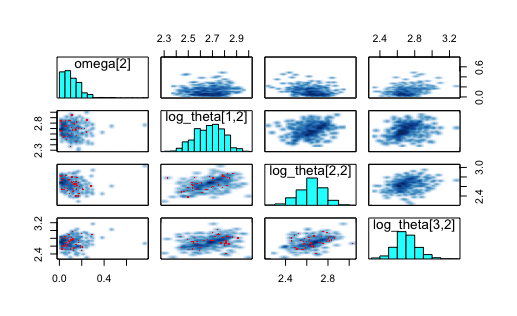
\includegraphics[width=9cm]{../figures/twoCptPairs2}
%  \end{center}
%\end{frame}

\begin{frame}

  \textit{\textcolor{MRGGreen}{Exercise 6}:
    Reparametrize the two compartment population model and fit it.}
    \begin{itemize}
      \item First, work out the appropriate parametrization. You should start with
      $\log \theta_i \sim \mathrm{Normal}(\theta_{\mathrm{pop}, i}, \omega)$
      \item Write, fit, and check the inference (run 100 chains).
      \item What kind of predictive checks can we do?
    \end{itemize}

\end{frame}

\begin{frame}
  Need:
  \begin{itemize}
    \item predictions at an individual level
    \item predictions at a population level
  \end{itemize}

  \ \\ \ \\
  As always, this comes down to properly writing the data generating process
  in the generated quantities block.

\end{frame}

\begin{frame}
  \frametitle{Individual predictions}
  
  \begin{center}
    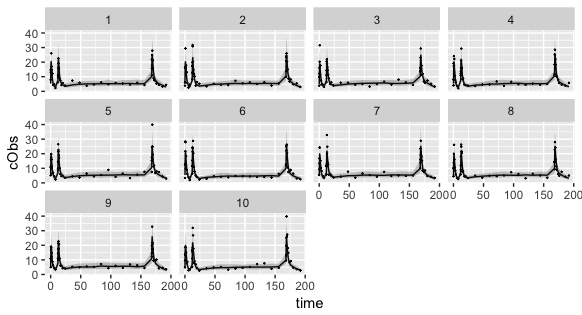
\includegraphics[width = 10cm]{../figures/PredictionPatient.png}
  \end{center}
  
\end{frame}

\begin{frame}
  \frametitle{Population predictions}

  \begin{center}
    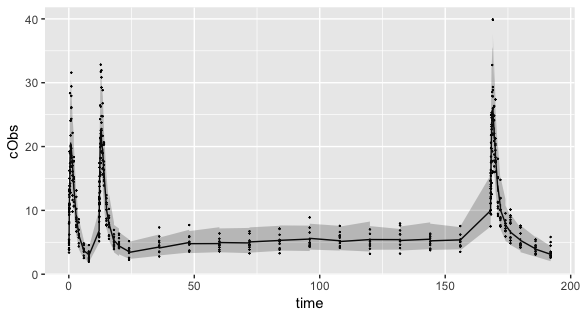
\includegraphics[width = 10cm]{../figures/PredictionPopulation.png}
  \end{center}

\end{frame}

\begin{frame}

  \begin{itemize}
    \item For a very good case study on hierarchical models, see,
    Bob Carpenter's \textit{Pooling with Hierarchical Models for Repeated Binary Trials}
   \item \url{https://mc-stan.org/users/documentation/ case-studies/pool-binary-trials.html}
 \end{itemize}

\end{frame}

\section{References}
\begin{frame}[allowframebreaks]{References}
\scriptsize
% \bibliographystyle{unsrt}
%\bibliographystyle{authoryear}
\bibliographystyle{apalike}
\bibliography{../ref}  
\end{frame}


\end{document}
